\documentclass{article}
\usepackage{graphicx} 
\usepackage[ddmmyyyy]{datetime}
\usepackage{titling}
\usepackage{listings}
\usepackage{xcolor}
\usepackage{wrapfig}

\colorlet{punct}{red!60!black}
\definecolor{background}{HTML}{EEEEEE}
\definecolor{delim}{RGB}{20,105,176}
\colorlet{numb}{magenta!60!black}

\lstdefinelanguage{json}{
    basicstyle=\fontsize{6}{5}\ttfamily,
    showstringspaces=false,
    breaklines=true,
    %frame=lines,
    %backgroundcolor=\color{background},
    literate=
     *{0}{{{\color{numb}0}}}{1}
      {1}{{{\color{numb}1}}}{1}
      {2}{{{\color{numb}2}}}{1}
      {3}{{{\color{numb}3}}}{1}
      {4}{{{\color{numb}4}}}{1}
      {5}{{{\color{numb}5}}}{1}
      {6}{{{\color{numb}6}}}{1}
      {7}{{{\color{numb}7}}}{1}
      {8}{{{\color{numb}8}}}{1}
      {9}{{{\color{numb}9}}}{1}
      {:}{{{\color{punct}{:}}}}{1}
      {,}{{{\color{punct}{,}}}}{1}
      {\{}{{{\color{delim}{\{}}}}{1}
      {\}}{{{\color{delim}{\}}}}}{1}
      {[}{{{\color{delim}{[}}}}{1}
      {]}{{{\color{delim}{]}}}}{1},
}

\renewcommand{\dateseparator}{.}

\DeclareFontFamily{\encodingdefault}{\ttdefault}{\hyphenchar\font=`\/}

\pretitle{
    \begin{center}
        
\includegraphics[width=10cm, height=10cm, keepaspectratio]{epfl.png}\\[\bigskipamount]
}
\posttitle{\end{center}}

\title{User Privacy Behavior Change in Instagram} 
\author{Romain \textsc{Choukroun}} 
\date{\today}

\begin{document}

\maketitle

\newpage
\tableofcontents

\newpage
\section{Abstract}
    Privacy has always been and always will be a cornerstone of society, maybe first layed out by Aristotle as the "private" sphere opposed to the "public" sphere. 
    \\Through history, the concept of privacy has not really changed, it still is about collecting information, disclosing them and intrusion in personal spaces. What has changed is the domain on which it applies, in fact, with the birth of so many social networks and media sharing platforms, the mere concept of privacy is somewhat overshadowed by the growing interest in said technologies for the grand public.
    \\Users seem to be less concerned about privacy matters when using such tools. This privacy-related behavior is influenced by several factors, which are what we focused on during this project.
    \\As one of the main media sharing networks, instagram was an obvious choice for that purpose. More precisely, we want to take a look at which factors can affect each user, and to what extent. Will the attitude of users change depending on who they start to follow ? On the content they consume ? On the overall trend of their feed ?
    \\In order to study such a behavior, we split the project into two tasks. First off continuously collect instagram posts by users. Then build a photo analysis tool capable of understanding the photo content opposed to just the context set by the different tags, sections, comments.
    \\It is the latter that I will elaborate on during this report.

\newpage
\section{Introduction}
    \subsection{Motivation}
        The average instagram user will most likely be a young person with a relatively small understanding of privacy-related issues concerning his/her content or his/her behavior, hence the importance of raising awareness to the public. 
        \\As a consequence, we cannot stress enough the urgency of the matter. Without privacy, there would not be any limit on the power that one would detain if he were to gain access to private information. The ability to change and have a second chance at an online life, the freedom of speech and thought are also key concepts enabled by privacy.
    \subsection{Analyzing an input}
        The idea behind the tool we wrote is to gather as much information as possible about a picture, an image or multiple of them fed as input. The output consists of a JSON containing said information. We focus on a certain number of features to get a good grasp of the context in which the picture was taken. The next figure is a screenshot from out web demo, it highlights some of them. 
        \begin{figure}[h]
            \centering
            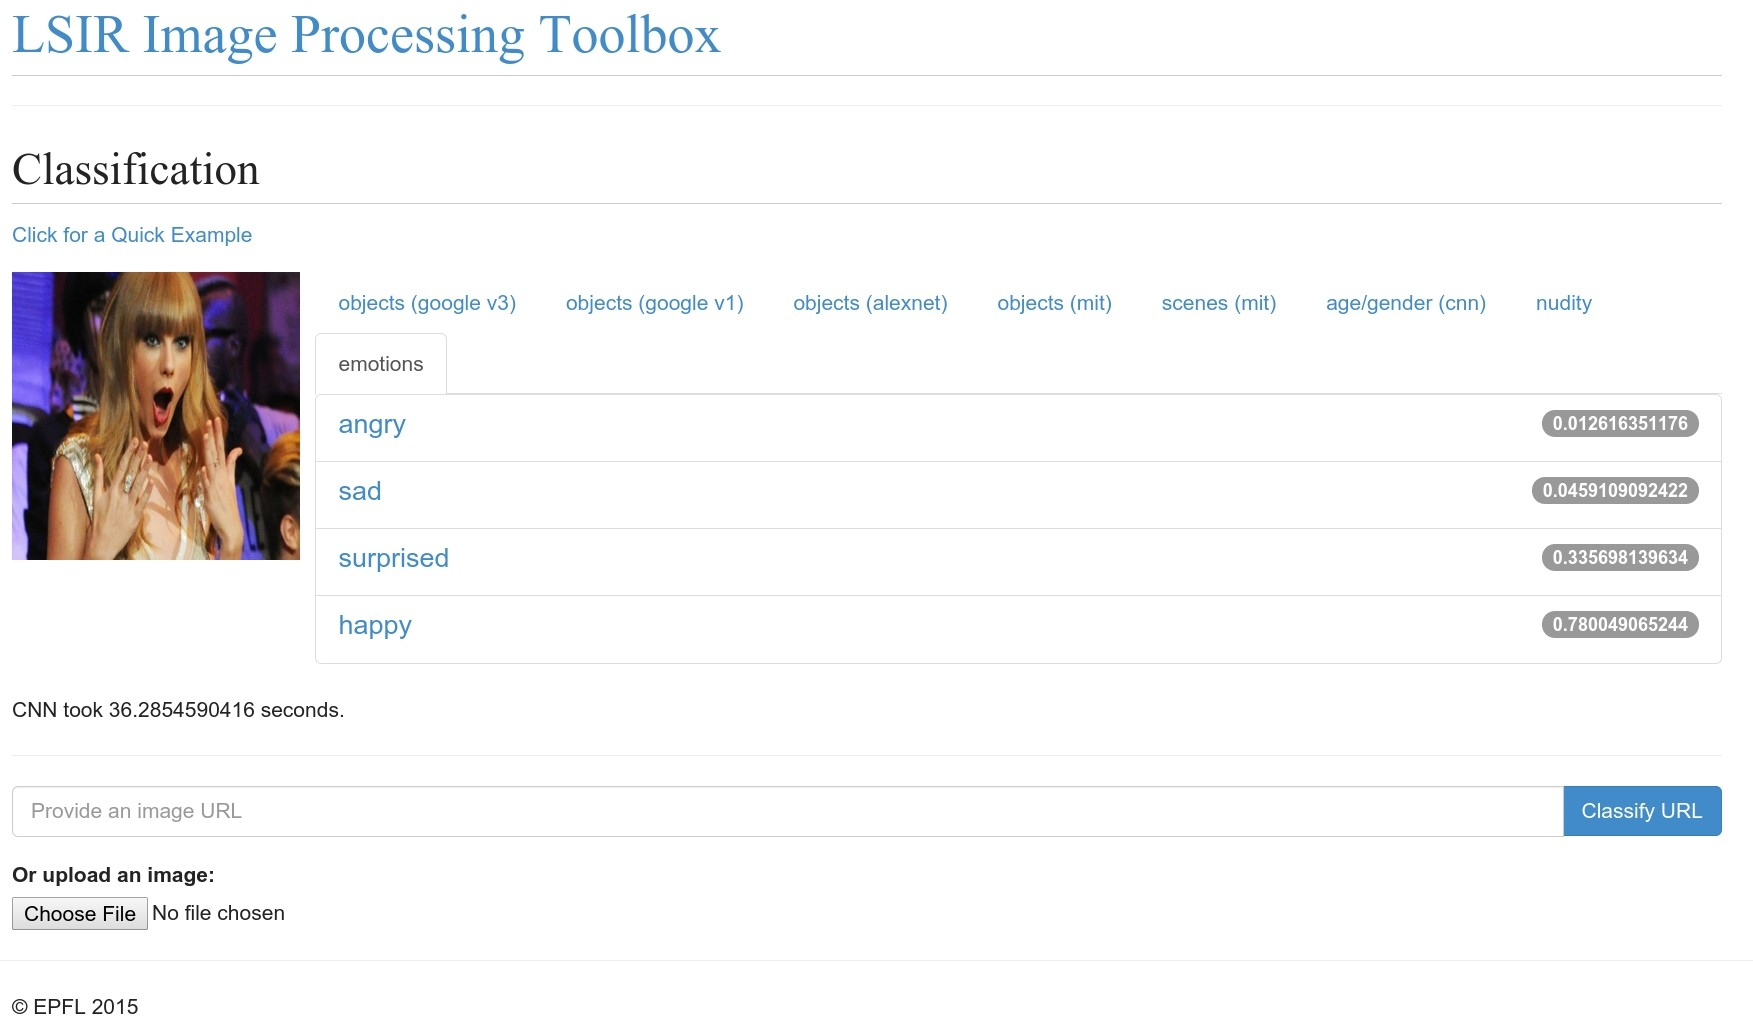
\includegraphics[scale=0.18]{emotions.jpg}
            \caption{Web demo focusing on emotion detection}
          \label{fig:emotions}
        \end{figure}
        \\As the aim of the project is analyzing privacy-related behavior of users, and not refining computer vision techniques, we did not develop the corresponding analysis tools from scratch, but used existing open-source frameworks and machine learning models.

\newpage
\section{Code Architecture}
    \subsection{Early Choices}
        The most obvious choice of language if one wants to run a machine learning heavy program as a backend is Python. In fact, a lot of machine learning open-source frameworks or projects are written in/or have an interface to Python. Which makes it easy to build a tool using all of these parts with almost a single language.
        \\Moreover, the Caffe framework \cite{caffe} has been our go-to deep learning tool when going about scene detection, object recognition and a part of age and gender.
        Concerning the other features, we found a lot of exciting open-source work on GitHub like the Pornographic images jacking algorithm (PIJA) \cite{pija} which analyzes the pixels of a picture in order to classify it as nudity or not. For face detection we used the OpenCV wrapper in Python using Haar Cascades \cite{haar}.
        \\Around the end of 2015, Google released TensorFlow \cite{tensor} which we implemented for scenes and objects recognition considering its accuracy.
        Some of the results of the age and gender models from Caffe were not convincing enough, so we decided to add the output from the OpenBiometrics \cite{openbr} age and gender classifiers.
        And last but not least, the emotions detection was drawn from an amazing library found on GitHub called clmtrackr \cite{clm}.
    \newpage
    \subsection{Output}
        In the following figure, you can see an image and its output. We chose the JSON format as it's the most widely used and easy to parse for human-readable data exchange. 
        \begin{lstlisting}[language=json,firstnumber=1]
{
  "file_path":"Photo_analysis/images/vase.jpg",
  "analysis":{
    "face_detection":"/Photo_analysis/results/vase.jpg",
    "scenes_and_objects":{
      "scenes_and_objects":{
        "imagenet":[ 
            {"confidence":"0.9566341639", "result":"vase"}, {"confidence":"0.0160881840", "result":"pitcher"},
            {"confidence":"0.0080848709", "result":"soap dispenser"}, {"confidence":"0.0075505734", "result":"perfume"},
            {"confidence":"0.0026656857", "result":"water jug"}, {"confidence":"0.0021058426", "result":"pop bottle"},
            {"confidence":"0.0012318835", "result":"Windsor tie"} 
          ],
        "tensorflow":[ 
            {"confidence":"0.962913", "result":"vase"}, {"confidence":"0.0103573", "result":"pitcher, ewer"},
            {"confidence":"0.0024912", "result":"water jug"}, {"confidence":"0.00140067", "result":"perfume, essence"},
            {"confidence":"0.000463179", "result":"table lamp"} 
          ],
        "mit_places_objects":[ 
            {"confidence":"0.7677739859", "result":"vase"}, {"confidence":"0.0802639052", "result":"pitcher, ewer"},
            {"confidence":"0.0578956716", "result":"Windsor tie"}, {"confidence":"0.0182715617", "result":"sock"},
            {"confidence":"0.0084599126", "result":"perfume, essence"}, {"confidence":"0.0064541521", "result":"coil, spiral, volute, whorl, helix"},
            {"confidence":"0.0056061158","result":"wool, woolen, woollen"} 
          ],
        "google_net":[ 
            {"confidence":"0.9952572584", "result":"vase"}, {"confidence":"0.0035603321", "result":"pitcher"},
            {"confidence":"0.0004608589", "result":"perfume"}, {"confidence":"0.0004501561", "result":"goblet"} 
          ]
      },
      "mit_places_scenes":[
          {"confidence":"0.0000339708", "result":"g/gift_shop"}, {"confidence":"0.0000232988", "result":"a/art_gallery"},
          {"confidence":"0.0000095298", "result":"a/aquarium"}, {"confidence":"0.0000079828", "result":"c/clothing_store"},
          {"confidence":"0.0000045859", "result":"c/candy_store"}, {"confidence":"0.0000036292", "result":"m/museum/indoor"},
          {"confidence":"0.0000014239", "result":"b/bakery/shop"}
        ]
    },\end{lstlisting}
    \begin{wrapfigure}[0]{r}{0.9\textwidth}
      \begin{center}
       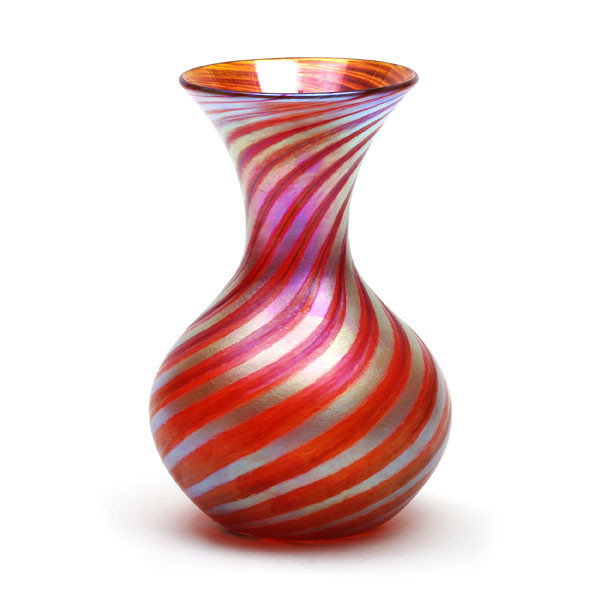
\includegraphics[scale=0.15]{vase.jpg}
      \end{center}
      \caption{The analyzed picture}
    \end{wrapfigure}
  \begin{lstlisting}[language=json,firstnumber=1]
    "age_and_gender":{
      "cnn":{
        "gender":"0",
        "age":{
          "max":"0",
          "min":"0"
        }
      },
      "open_br":{
        "gender":"0",
        "age":"0"
      }
    },
    "emotions":{
      "angry":"0",
      "sad":"0",
      "surprised":"0",
      "happy":"0"
    },
    "nudity":"False"
  }
}
        \end{lstlisting}
    \subsection{Data Storing}
        As the project is about data collection and analysis, we needed a way to store results. MongoDB \cite{mongo} seemed like the perfect document-oriented database since it focuses on storing Objects in JSON documents. Using MongoDB through the PyMongo module for Python \cite{pym}, we can easily link the first part of the project (data collection) with the second part (data analysis) as well as maybe a future user interface. 
        For the sake of privacy, JSONs obtained through running the web demo shall not be stored.
\section{Classifiers}
    Each prediction is given as the output of a particular classifier, here we will discuss them in details. We opted to run multiple classifiers for each category in order to have a wider array of predictions, hereby tightening the choices. Given an input, each classifier yields one or multiple predictions for his own feature which we then sort from most probable to least and select.
    \subsection{Scenes and Objects}
        All the scenes and objects classifiers are based on deep learning and use available pretrained models.
        The ImageNet \cite{imnet}, Hybrid-CNN MIT \cite{hybrid} and BVLC GoogleNet models are all caffe models found on the Model-Zoo \cite{zoo}. 
        \\While ImageNet and GoogleNet focus on the objects, the Hybrid-CNN is, as named, an hybrid between scenes and objects. Consequently, it will yield predictions for both objects and scenes which are then sorted and classified as one or the other. This means that, for example, if we classify a vase image, then the prediction "vase" as an object will be higher than, say, the prediction "gift shop" as a scene for this case. Since we can only compare scenes predictions with other scenes predictions, we group them together and output a second list of results, only for the scenes this time (see the JSON output in 3.2).
        \\Google then released their TensorFlow \cite{tensor} library that we implemented as the TensorFlow classifier which, as you can see, gives also great results on objects.
        [GRAPH OF RESULTS PER MODEL CONTAINING IMAGENET HYBRID GOOGLENET TENSORFLOW]
    \subsection{Age and Gender}
        The output of an age and gender model is usually simple, a boolean to qualify the gender and an interval concerning the age.
        The last of the caffe models we used is called AgeGenderDeepLearning \cite{age}, also available in the Model Zoo. It classifies the age and gender of a detected face using machine learning and a pretrained model.
        \\OpenBiometrics \cite{openbr} is the other option concerning age and gender. It is also based on machine learning and OpenCV \cite{opencv}. We use the commandline interface through Python in order to classify a given portrait.
        \\The accuracy of each model is as follows:
        [GRAPH RESULTS PER MODEL CONTAINING CNN AGE GENDER AND OPENBR]
    \subsection{Face Detection}
        We detect faces using OpenCV and a Haar Cascade file trained specifically for face detection, it yields the same picture as the original file with a green rectangle surrounding the detected faces. The path to this output file is given in the JSON.
    \subsection{Nudity}
        Nudity detection is done through an open-source library found on GitHub called PIJA \cite{pija}, first intended to prove that a malware could detect and steal homemade adult content from a remote machine. PIJA gave us good results in testing compared to other free libraries and being written in Python, it was easy to implement into a building block of our tool. 
        \\It is based on skin pixel detection using OpenCV \cite{opencv}, by first finding a skin mask after converting the input as a Numpy array, and finally simply counting the proportion of skin pixels compared to the others.
    \subsection{Emotions}
        Concerning emotion detection, the really good clmtrackr JavaScript library found on GitHub \cite{clm} was an obvious choice. It works by tracking a facial model in a video or image and recording the coordinate position of each number as follows. 
        \begin{figure}[h]
            \centering
            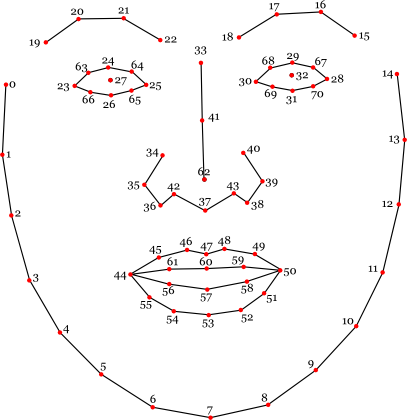
\includegraphics[scale=0.7]{clm.png}
            \caption{Clmtrackr's facial numbered model}
        \end{figure}
        \newpage
        Their demo is pretty impressive \cite{clmdemo}, which is what convinced us. Since the library is written in JavaScript we have to run it in a browser, thanks to the selenium WebDriver API \cite{web} we can power up a headless browser in Python with a webserver written in NodeJS \cite{node} running in background.
        \\So what the code does is start a simple NodeJS web server and then run the JavaScript  code needed to classify the emotions of the input into PhantomJS (WebDriver) \cite{phan}. We are then able to output the emotions as a JSON with, for now, four features: angry, happy, surprised, and sad each having its own confidence level. If no face is found in the picture, each said confidence level will be, by default, set to 0.

\newpage
\section{Future Work}
    There is still a lot of work to be done, which is really exciting, but here are some of the most obvious optimizations. 
    \\First of all, we need to add parallelization. In fact, performance is not the worst but running on a laptop CPU without any parallelization, and no GPU, it takes around 15 seconds to fully classify one image. This time should be reduced to around 1 second by parallel processing and multiprocessing in Python. 
    \\Since Google came out with TensorFlow \cite{tensor}, it might be needed to switch our models to it. It is also crucial to start working more on a better detection of faces, and maybe seperate the emotion classification of each detected face. 
    \\We also have a web demo for the project, as you could see in Figure \ref{fig:emotions} \cite{demo}, and need to optimize it more for concurrent use. There should also be more flexibility: provide a set of models to choose from and maybe refine the user interface. 
    \\An activity model will be implemented soon, it is still in training on the LSIR cluster. 
    Detecting activities is a huge step in the direction of better understanding the context of a picture. 
    \\A ton more features could be implemented to complete such a tool, like Image Captioning and Optical Character Recognition.
\section{Conclusion}
    In this report, we presented you an image analysis tool capable of classifying an input with a set of specific features in mind like the scenes, objects and much more. We hope that it will help the LSIR lab \cite{lsir} and the community to continue working on privacy-related issues, may they dissapear one after the other. With the work left to be done in the machine learning field, the accuracy of such predictions and classifications will not stop growing.
\section{Credits}
This Bachelor project was offered to me by my supervisor Hamza Harkous and exceeded all of my expectations. I would like to thank Hamza very much for all of his help and advice on different implementation matters and also for helping me setup my environment. It was a real pleasure to work with him and the LSIR lab in general.
\newpage
\begin{thebibliography}{20}
\bibitem{caffe} 
Caffe framework,
\\\texttt{http://caffe.berkeleyvision.org/}
 
\bibitem{pija} 
Pija GitHub,
\\\texttt{https://github.com/alcuadrado/pija/}
 
\bibitem{haar} 
Face detection using Haar Cascades,
\\\texttt{http://opencv-python-tutroals.readthedocs.org/en/latest/py\_tutorials/py\_objdetect/py\_face\_detection/py\_face\_detection.html}

\bibitem{tensor} 
TensorFlow from Google,
\\\texttt{https://www.tensorflow.org/}

\bibitem{openbr} 
OpenBiometrics,
\\\texttt{http://openbiometrics.org/}

\bibitem{clm} 
Clmtrackr GitHub,
\\\texttt{https://github.com/auduno/clmtrackr/}

\bibitem{mongo} 
MongoDB,
\\\texttt{https://www.mongodb.org/}

\bibitem{pym} 
PyMongo Python distribution,
\\\texttt{https://api.mongodb.org/python/current/}

\bibitem{zoo} 
Caffe Model Zoo,
\\\texttt{https://github.com/BVLC/caffe/wiki/Model-Zoo/}

\bibitem{imnet} 
Imagenet model,
\\\texttt{https://gist.github.com/mavenlin/d802a5849de39225bcc6/}

\bibitem{hybrid} 
Hybrid-CNN,
\\\texttt{http://places.csail.mit.edu/}

\bibitem{age} 
Age and Gender model,
\\\texttt{http://www.openu.ac.il/home/hassner/projects/cnn\_agegender/}

\bibitem{opencv} 
OpenCV,
\\\texttt{http://opencv.org/}

\bibitem{clmdemo} 
Clmtrackr's emotion detection demo,
\\\texttt{https://auduno.github.io/clmtrackr/examples/clm\_emotiondetection.html}

\bibitem{web} 
Slenium Webdriver API,
\\\texttt{http://www.seleniumhq.org/docs/03\_webdriver.jsp}

\bibitem{node}
NodeJS,
\\\texttt{https://nodejs.org/en/}

\bibitem{phan}
PhantomJS,
\\\texttt{http://phantomjs.org/}

\bibitem{demo}
Privyseal Image Processing Toolbox (only accessible through EPFL's VPN),
\\\texttt{http://privyseal.epfl.ch:5000/}

\bibitem{lsir}
EPFL LSIR lab,
\\\texttt{http://lsir.epfl.ch/research/themes/}

\end{thebibliography}

\end{document}